\section{When agents replace human gate work}
\label{sec:substitution}

\paragraph{A complete account.}
At fixed case volume $\lambda>0$, let $h_0>0$ be mean baseline handling hours. A frozen routing
rule sends a fraction $q$ of cases to substantive human exception handling. Let $h_E$ be
complete human hours on those cases, $h_R$ ordinary-path human review, and $h_W$ additional
rework per case. Recurring human upkeep is $B_H$ in the baseline and $B_A$ after deployment.
Then
\begin{equation}
 L_H=\lambda h_0+B_H,\qquad
 L_A=\lambda\{qh_E+(1-q)h_R+h_W\}+B_A.
 \label{eq:short-hours}
\end{equation}
Exceptions include their preliminary review; ordinary review includes mandatory signatures
and expected sampled audits. Rework, downstream repair, supplier effort, evaluation, and
policy maintenance are allocated once across the common process boundary. Changing a
department or job title does not remove the hours. Initial implementation is reported
separately for a transition-cost calculation; recurring adaptation belongs in $B_A$.

The fraction of cases retained by humans is generally different from the fraction of work
retained. Let $T$ be baseline handling time, $J$ indicate exception routing, and
$h_0=\mathbb E[T]$. Define the residual's baseline labor share
$\phi=\mathbb E[TJ]/h_0$, its effort multiplier
$\eta=h_E/\mathbb E[T\mid J=1]$, and the ordinary group's retained review fraction
$\mu=h_R/\mathbb E[T\mid J=0]$. Assume both conditional baseline means are positive and
$0<q<1$; Equation~\eqref{eq:short-hours} covers the other cases. With
$r=h_W/h_0$ and $b_s=B_s/(\lambda h_0)$, the workload ratio is
\begin{equation}
 \rho:=\frac{L_A}{L_H}
 =\frac{\phi\eta+(1-\phi)\mu+r+b_A}{1+b_H}.
 \label{eq:short-rho}
\end{equation}
This is an accounting identity, not an estimated effect of agents.

\begin{proposition}[Selection and the substitution frontier]
\label{prop:short-frontier}
Let $T\ge0$ be integrable with positive mean, and let
$e(t)=\Pr(J=1\mid T=t)$. Under the definitions above,
\begin{equation}
 \phi=q+\frac{\operatorname{Cov}(T,e(T))}{h_0}.
 \label{eq:short-selection}
\end{equation}
Thus routing that is nondecreasing in baseline effort retains at least as much baseline
labor as its share of cases. For any target fractional workload reduction $d\in[0,1]$,
achieving $L_A\le(1-d)L_H$ is equivalent to
\begin{equation}
 \phi\eta+(1-\phi)\mu+r+b_A\le(1-d)(1+b_H).
 \label{eq:short-target}
\end{equation}
\end{proposition}
\begin{proof}
Conditional expectation gives $\mathbb E[TJ]=\mathbb E[Te(T)]$. Expanding the covariance
and using $\mathbb E[e(T)]=q$ proves Equation~\eqref{eq:short-selection}. For independent
copies $T,T'$, twice this covariance is
$\mathbb E[(T-T')(e(T)-e(T'))]$, which is nonnegative when $e$ is nondecreasing.
Splitting $h_0$ between the two routing groups yields
$qh_E/h_0=\phi\eta$ and $(1-q)h_R/h_0=(1-\phi)\mu$.
Substitution into Equation~\eqref{eq:short-hours} proves
Equation~\eqref{eq:short-rho}; multiplication by its positive denominator gives the target
condition.
\end{proof}

The practical consequence is that an agent success rate cannot be read as the percentage
of human labor removed. For example, 20\% of cases retain 40\% of baseline labor when their
baseline handling time is twice the overall mean. If their post-deployment effort rises by
50\%, those exceptions alone consume 60\% of baseline handling hours. This is the
mechanism by which a small exception queue can prevent a large workforce reduction.

\paragraph{Reliability consumes the same budget.}
If erroneous accepted outputs occur on a fraction $p$ of all cases and cause additional human
repair averaging $h_C$ hours conditional on such an error, their contribution to $r$ is
$p h_C/h_0$, counted once.
This links execution reliability to the labor target, but does not make low repair cost a
quality guarantee. An undetected harmful error is unacceptable even if it consumes no repair
hours. Strict benchmark failures, human escalations, and erroneous accepted outputs are
different events; the experiments do not measure deployment values of $q$ or $h_C$.

\paragraph{Coverage does not determine required labor.}
The extended manuscript's reproducible synthetic example allocates 140 baseline FTE
across nine governance populations, at 120 useful hours per FTE per month. Each population
has 100 pooled review visits, exception fractions from 0.16 to 0.33, and exception baseline
means twice its overall mean. The workload-weighted exception fraction is 23.43\%, while
the groups retain 46.86\% of baseline labor. With these partitions unchanged, the
calculated requirements are shown in Figure~\ref{fig:labor}.
The scenario parameters $(\eta,m,h_W,B_A)$ are respectively
$(0.5,0.10,0,0)$, $(1,0.10,0,120)$, $(1,0.10,0.5,120)$, and
$(1.5,0.35,2,240)$. Here $h_R=m h_0$, so $m$ differs from the group-relative $\mu$;
$h_W$ is hours per case and $B_A$ hours per population per month. Baseline upkeep is zero.
The paired population vectors are baseline FTE $(10,10,30,20,10,25,15,10,10)$ and
$q=(0.22,0.33,0.18,0.16,0.22,0.24,0.26,0.33,0.33)$.
\begin{figure}[!htb]
\centering
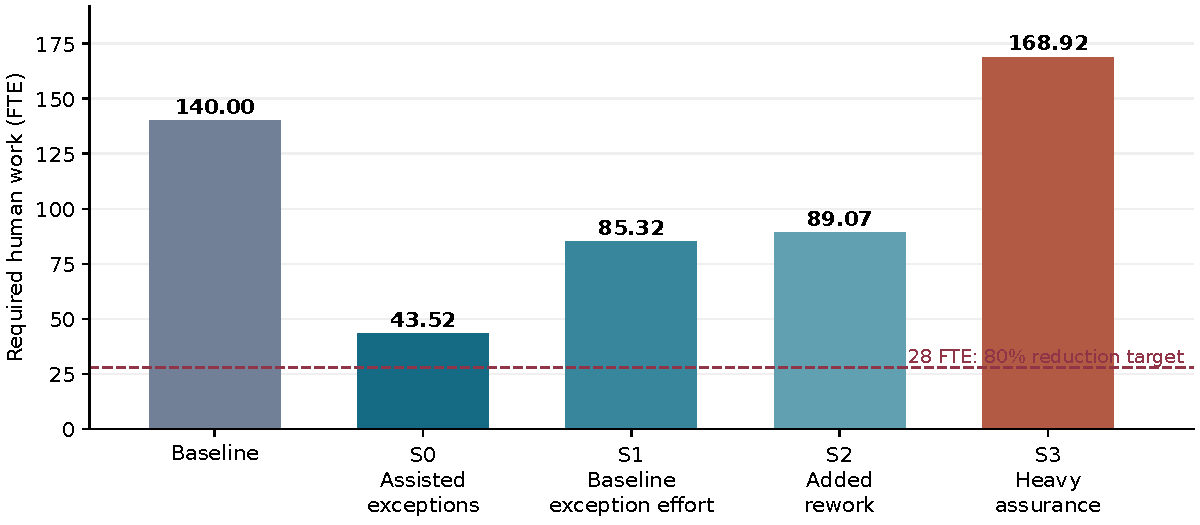
\includegraphics[width=0.88\linewidth]{figures/fig_labor_scenarios.pdf}
\caption{Illustrative human-work requirements with the same case partition: baseline 140 FTE;
four operating assumptions produce 43.52, 85.32, 89.07, and 168.92 FTE. The dashed line is the
author's 80\% reduction target, not a fitted forecast. Parameters and calculation are released.}
\label{fig:labor}
\end{figure}
These are sensitivity calculations using declared assumptions, not measurements or
forecasts. The comparison establishes a useful non-identification result: even fixed
coverage and a fixed baseline case partition do not determine the sign of the labor
effect. Their associated quality is not estimated. A deployment must measure both the
contract outcomes and the complete account to identify whether execution has actually
been substituted at acceptable quality.
None of these four scenarios reaches an 80\% reduction. With $\phi\simeq0.4686$ and no other
residual burden, that target already requires $\eta\le0.20/\phi\simeq0.427$.
Thus the forecast requires further reduction in exception effort or in its retained labor
share, even before allowing for ongoing review and support.

\paragraph{From required work to staffing.}
At fixed useful capacity $K>0$, required workload-equivalent FTE equal $L/K$. Under the
additional assumptions of interchangeable workers, target utilization $0<u\le1$, no separate
coverage constraint, and staffing chosen to minimize labor cost, required headcount is
$\lceil L/(uK)\rceil$. Reducing required hours then removes posts when this integer crosses
a staffing threshold. Redeployment or increased demand can absorb the released capacity;
they do not make execution of the old tasks indispensable again. For a finite collection
of gates with bounded visit counts, vanishing human case effort leaves a support floor
$B_A/K$; zero total human labor further requires that this support work be eliminated or
automated. These are explicit conditions for displacement, not a claim that current
benchmark performance has already satisfied them.
